%%%%%%%%%%%%%%%%%%%%%%%%%%%%%%%%%%%%%%%%%%%%%%%%%%%%%%%%%%%%%%%%%%%%%%%%%%%%%%%%%%
\begin{frame}[fragile]\frametitle{}
\begin{center}
{\Large RAG Advanced Concepts}
\end{center}
\end{frame}

%%%%%%%%%%%%%%%%%%%%%%%%%%%%%%%%%%%%%%%%%%%%%%%%%%%%%%%%%%%%%%%%%%%%%%%%%%%%%%%%%%
\begin{frame}[fragile]\frametitle{}
\begin{center}
{\Large Model Optimization}
\end{center}
\end{frame}


%%%%%%%%%%%%%%%%%%%%%%%%%%%%%%%%%%%%%%%%%%%%%%%%%%%%%%%%%%%%%%%%%%%%%%%%%%%%%%%%%%
\begin{frame}[fragile]{Deploying Large Language Models}
  \begin{itemize}
    \item Challenge: LLMs' size and computational demands in production.
    \item Optimisation strategies crucial for cost-effective deployment.
  \end{itemize}
\end{frame}

%%%%%%%%%%%%%%%%%%%%%%%%%%%%%%%%%%%%%%%%%%%%%%%%%%%%%%%%%%%
\begin{frame}[fragile]\frametitle{Model Compression}


		\begin{center}
		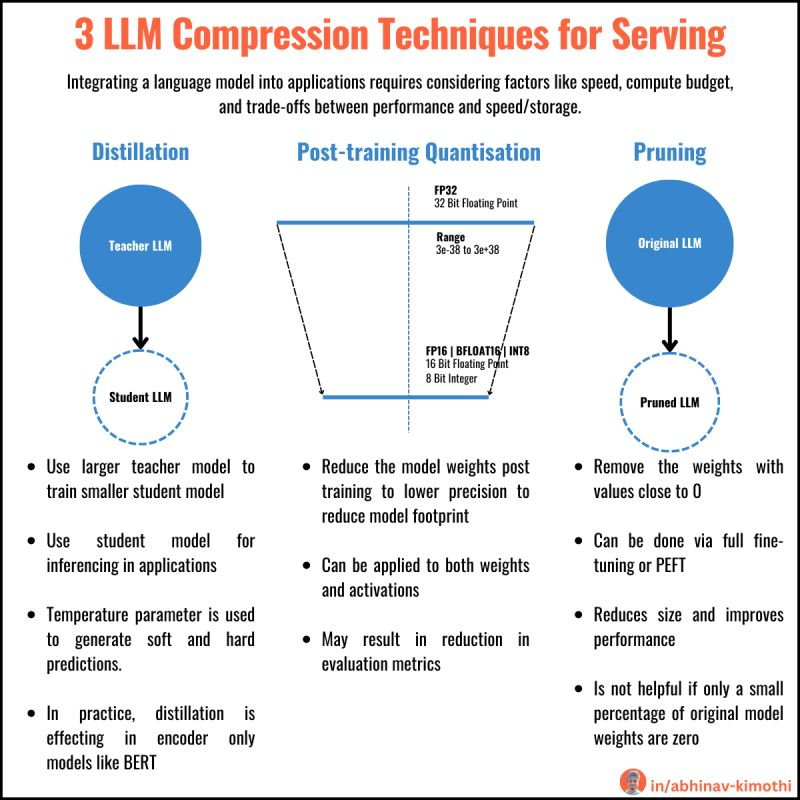
\includegraphics[width=0.6\linewidth,keepaspectratio]{rag16}
		\end{center}

{\tiny (Ref: Knowledge Brain RAG - Abhinav  Kimothi)}

\end{frame}


%%%%%%%%%%%%%%%%%%%%%%%%%%%%%%%%%%%%%%%%%%%%%%%%%%%%%%%%%%%%%%%%%%%%%%%%%%%%%%%%%%
\begin{frame}[fragile]{Model Quantisation}
  \begin{itemize}
    \item Converts parameters and activations to lower precision data types.
    \item Reduces memory and computation requirements.
    \item Increases inference speed (2-4x) using int8 arithmetic.
    \item Approaches: post-training, quantisation-aware training, hybrid quantisation.
    \item Tradeoff analysis needed between reduced precision and model accuracy.
  \end{itemize}
\end{frame}

%%%%%%%%%%%%%%%%%%%%%%%%%%%%%%%%%%%%%%%%%%%%%%%%%%%%%%%%%%%%%%%%%%%%%%%%%%%%%%%%%%
\begin{frame}[fragile]{Model Pruning}
  \begin{itemize}
    \item Removes redundant parameters to reduce size and complexity.
    \item Weight pruning removes individual weights based on magnitude.
    \item Neuron pruning removes entire neurons based on importance.
    \item Requires fine-tuning for maintaining accuracy.
    \item Approaches: post-training, iterative pruning.
  \end{itemize}
\end{frame}

%%%%%%%%%%%%%%%%%%%%%%%%%%%%%%%%%%%%%%%%%%%%%%%%%%%%%%%%%%%%%%%%%%%%%%%%%%%%%%%%%%
\begin{frame}[fragile]{Model Distillation}
  \begin{itemize}
    \item Transfers knowledge from large "teacher" to smaller "student" model.
    \item Student mimics teacher's outputs using labeled data and teacher probabilities.
    \item Enhances efficiency while approximating teacher accuracy.
    \item Includes knowledge distillation, self-distillation, ensemble distillation.
  \end{itemize}
\end{frame}

%%%%%%%%%%%%%%%%%%%%%%%%%%%%%%%%%%%%%%%%%%%%%%%%%%%%%%%%%%%%%%%%%%%%%%%%%%%%%%%%%%
\begin{frame}[fragile]{Combined Optimisation Techniques}
  \begin{itemize}
    \item By combining quantisation, pruning, and distillation:
    \item Unlock benefits of large language models.
    \item Control deployment costs and energy consumption.
  \end{itemize}
\end{frame}


%%%%%%%%%%%%%%%%%%%%%%%%%%%%%%%%%%%%%%%%%%%%%%%%%%%%%%%%%%%%%%%%%%%%%%%%%%%%%%%%%%
\begin{frame}[fragile]\frametitle{}
\begin{center}
{\Large Multimodal Models}
\end{center}
\end{frame}


%%%%%%%%%%%%%%%%%%%%%%%%%%%%%%%%%%%%%%%%%%%%%%%%%%%%%%%%%%%%%%%%%%%%%%%%%%%%%%%%%%
\begin{frame}[fragile]{Multimodal AI Models}
    \begin{itemize}
        \item Most AI models historically limited to a single modality (text, images, or video).
        \item Recent progress in handling multiple modalities, especially text and images.
    \end{itemize}
\end{frame}

%%%%%%%%%%%%%%%%%%%%%%%%%%%%%%%%%%%%%%%%%%%%%%%%%%%%%%%%%%%%%%%%%%%%%%%%%%%%%%%%%%
\begin{frame}[fragile]{Features of Multimodal RAG}
    \begin{itemize}
        \item Ability to query/prompt in one or more modalities (e.g., text and images).
        \item Search and retrieve not only text but also images, tables, audio files related to the query.
        \item Ability to generate text, image, video, etc., irrespective of the input mode(s).
    \end{itemize}
\end{frame}

%%%%%%%%%%%%%%%%%%%%%%%%%%%%%%%%%%%%%%%%%%%%%%%%%%%%%%%%%%%%%%%%%%%%%%%%%%%%%%%%%%
\begin{frame}[fragile]{Emergent Approaches in Multimodal RAG}
    \begin{itemize}
        \item Using multimodal embeddings like CLIP.
        \item Using LMMs to generate image captions and using text embeddings.
    \end{itemize}
\end{frame}

%%%%%%%%%%%%%%%%%%%%%%%%%%%%%%%%%%%%%%%%%%%%%%%%%%%%%%%%%%%%%%%%%%%%%%%%%%%%%%%%%%
\begin{frame}[fragile]{Multimodal Embeddings in RAG Workflow}
    \begin{itemize}
        \item \textbf{Multimodal Embeddings (e.g., CLIP):} Used for embedding both images and text.
        \item \textbf{Query/Prompt:} User input initiates the process.
        \item \textbf{Retrieved Context:} User query retrieves context (images and/or text).
        \item \textbf{LMM (Language Model):} Context, along with the prompt, passed to the Language Model.
        \item \textbf{Multimodal Response:} The Language Model generates the final response.
        \item \textbf{Indexing and RAG Pipelines:} Sequential steps involving embedding, retrieval, and response generation.
    \end{itemize}
\end{frame}


%%%%%%%%%%%%%%%%%%%%%%%%%%%%%%%%%%%%%%%%%%%%%%%%%%%%%%%%%%%
\begin{frame}[fragile]\frametitle{Multimodal RAG using Multimodal Embeddings}


		\begin{center}
		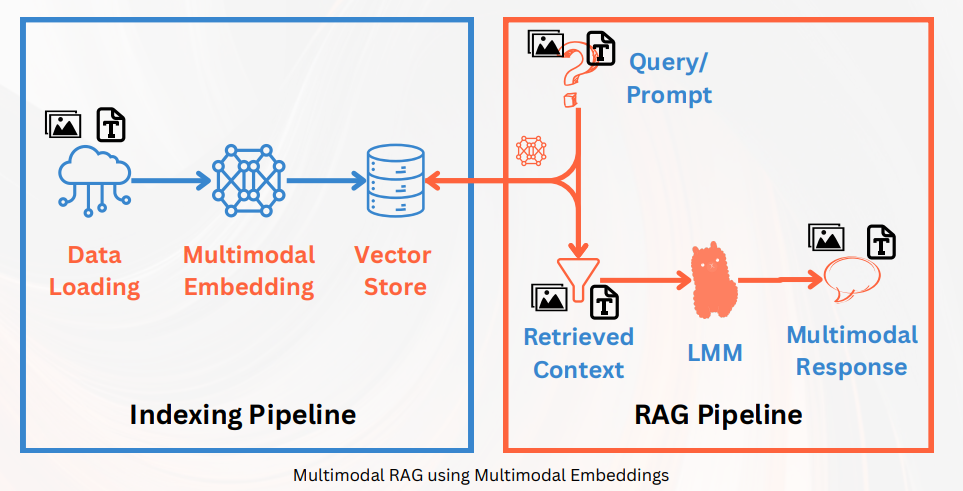
\includegraphics[width=0.6\linewidth,keepaspectratio]{rag12}
		\end{center}

{\tiny (Ref: Multimodal RAG - Abhinav  Kimothi)}

\end{frame}

%%%%%%%%%%%%%%%%%%%%%%%%%%%%%%%%%%%%%%%%%%%%%%%%%%%%%%%%%%%
\begin{frame}[fragile]\frametitle{CLIP : Contrastive Language-Image Pre-training}


		\begin{center}
		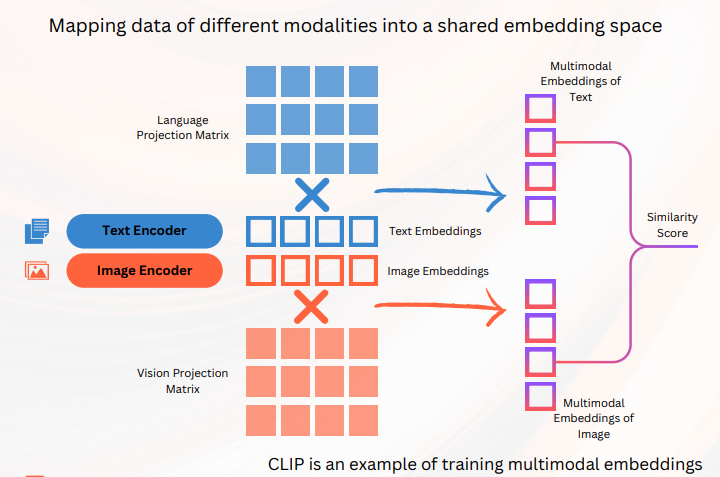
\includegraphics[width=0.6\linewidth,keepaspectratio]{rag13}
		\end{center}

{\tiny (Ref: Multimodal RAG - Abhinav  Kimothi)}

\end{frame}


%%%%%%%%%%%%%%%%%%%%%%%%%%%%%%%%%%%%%%%%%%%%%%%%%%%%%%%%%%%%%%%%%%%%%%%%%%%%%%%%%%
\begin{frame}[fragile]{MM-RAG Paper and Implementations}
    \begin{itemize}
        \item MM-RAG paper published in June 2023 provides insights into building a retriever for multimodal RAG.
        \item LangChain cookbook offers a simple implementation of multimodal RAG using a multiquery retriever and OpenAI GPT4V.
        \item LlamaIndex tutorial explains multimodal RAG implementation in detail.
    \end{itemize}
\end{frame}

%%%%%%%%%%%%%%%%%%%%%%%%%%%%%%%%%%%%%%%%%%%%%%%%%%%%%%%%%%%%%%%%%%%%%%%%%%%%%%%%%%
\begin{frame}[fragile]{Using LMMs for Text Summaries from Images}
    \begin{itemize}
        \item \textbf{Indexing:}
            \begin{itemize}
                \item LLM generates captions for images in the data.
                \item Captions and text summaries stored as text embeddings in a vector database.
                \item Maintains a mapping from image captions to image files.
            \end{itemize}
        \item \textbf{Generation:}
            \begin{itemize}
                \item User query with text and image.
                \item LLM generates image captions and embeddings.
                \item Search for text summaries and image captions; retrieve images based on relevant captions.
                \item Retrieved content passed to LMM with a prompt.
                \item LMM generates a multimodal response.
            \end{itemize}
    \end{itemize}
\end{frame}

%%%%%%%%%%%%%%%%%%%%%%%%%%%%%%%%%%%%%%%%%%%%%%%%%%%%%%%%%%%
\begin{frame}[fragile]{Using LMMs for Text Summaries from Images}


		\begin{center}
		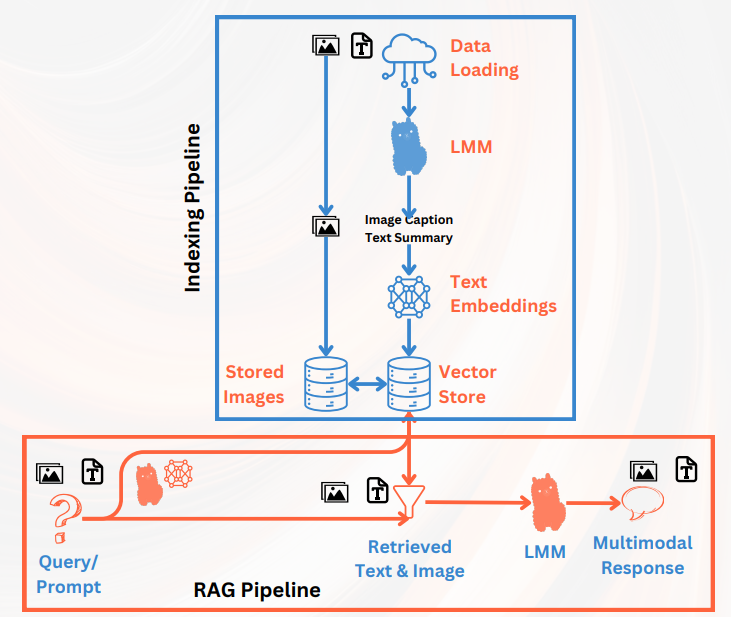
\includegraphics[width=0.6\linewidth,keepaspectratio]{rag14}
		\end{center}

{\tiny (Ref: Multimodal RAG - Abhinav  Kimothi)}

\end{frame}
